%%% LaTeX Template
%%% This template can be used for both articles and reports.
%%%
%%% Copyright: http://www.howtotex.com/
%%% Date: February 2011

%%% Preamble
\documentclass[paper=a4, fontsize=11pt]{scrartcl}	% Article class of KOMA-script with 11pt font and a4 format


\usepackage[protrusion=true,expansion=true]{microtype}				% Better typography
\usepackage{amsmath,amsfonts,amsthm}										% Math packages
\usepackage[pdftex]{graphicx}
\usepackage{siunitx}														% Enable pdflatex
%\usepackage{color,transparent}													% If you use color and/or transparency
\usepackage[hang, small,labelfont=bf,up,textfont=it,up]{caption}	% Custom captions under/above floats
\usepackage{epstopdf}																	% Converts .eps to .pdf
\usepackage{subfig}																		% Subfigures
\usepackage{booktabs}																	% Nicer tables


%%% Advanced verbatim environment
\usepackage{verbatim}
\usepackage{fancyvrb}
\DefineShortVerb{\|}								
\usepackage[ngerman]{babel}
\usepackage[utf8]{inputenc}


\usepackage{listings}
\usepackage{color}
 
 \usepackage{hyperref}

\definecolor{dkgreen}{rgb}{0,0.6,0}
\definecolor{gray}{rgb}{0.5,0.5,0.5}
\definecolor{mauve}{rgb}{0.58,0,0.82}
 
\lstset{ %
  language=Java,                % the language of the code
  basicstyle=\footnotesize\ttfamily, % Standardschrift
  numbers=left,                   % where to put the line-numbers
  numberstyle=\tiny\color{gray},  % the style that is used for the line-numbers
  stepnumber=1,                   % the step between two line-numbers. If it's 1, each line 
                                  % will be numbered
  numbersep=5pt,                  % how far the line-numbers are from the code
  backgroundcolor=\color{white},      % choose the background color. You must add \usepackage{color}
  showspaces=false,               % show spaces adding particular underscores
  showstringspaces=false,         % underline spaces within strings
  showtabs=false,                 % show tabs within strings adding particular underscores
  frame=single,                   % adds a frame around the code
  rulecolor=\color{black},        % if not set, the frame-color may be changed on line-breaks within not-black text (e.g. comments (green here))
           xleftmargin=17pt,
         framexleftmargin=17pt,
         framexrightmargin=5pt,
         framexbottommargin=4pt,
  tabsize=2,                      % sets default tabsize to 2 spaces
  captionpos=b,                   % sets the caption-position to bottom
  breaklines=true,                % sets automatic line breaking
  breakatwhitespace=false,        % sets if automatic breaks should only happen at whitespace
  title=\lstname,                   % show the filename of files included with \lstinputlisting;
                                  % also try caption instead of title
  keywordstyle=\color{blue},          % keyword style
  commentstyle=\color{dkgreen},       % comment style
  stringstyle=\color{mauve}\ttfamily,         % string literal style
  escapeinside={\%*}{*)},            % if you want to add LaTeX within your code
  morekeywords={*,...},              % if you want to add more keywords to the set
  deletekeywords={...}              % if you want to delete keywords from the given language
}

  %\captionsetup[lstlisting]{singlelinecheck=false, labelfont={blue}, textfont={blue}}
  \usepackage{caption}
\DeclareCaptionFont{white}{\color{white}}
\DeclareCaptionFormat{listing}{\colorbox[cmyk]{0.43, 0.35, 0.35,0.01}{\parbox{\textwidth}{\hspace{15pt}#1#2#3}}}


%%% Custom sectioning (sectsty package)
\usepackage{sectsty}								
\allsectionsfont{
\usefont{OT1}{bch}{b}{n}%					
	}

\sectionfont{%										% Change font of \section command
	\usefont{OT1}{bch}{b}{n}%					% bch-b-n: CharterBT-Bold font
	\sectionrule{0pt}{0pt}{-5pt}{0.8pt}%	% Horizontal rule below section
	}

\bibliographystyle{unsrt}
\usepackage[numbers]{natbib} 
%\usepackage[round]{natbib}

%%% Custom headers/footers (fancyhdr package)
\usepackage{fancyhdr}
\pagestyle{fancyplain}
\fancyhead{}														% No page header
\fancyfoot[C]{\thepage}										% Pagenumbering at center of footer
%\fancyfoot[R]{\small \texttt{HowToTeX.com}}	% You can remove/edit this line 
\renewcommand{\headrulewidth}{0pt}				% Remove header underlines
\renewcommand{\footrulewidth}{0pt}				% Remove footer underlines
\setlength{\headheight}{15pt}

%%% Equation and float numbering
\numberwithin{equation}{section}															% Equationnumbering: section.eq#
\numberwithin{figure}{section}																% Figurenumbering: section.fig#
\numberwithin{table}{section}																% Tablenumbering: section.tab#


%%% Title	
\title{ \vspace{-1in} 	\usefont{OT1}{bch}{b}{n}
		\huge \strut Masterprojekt \strut \\
		\Large \bfseries \ Android Anwendungen am praktischen Beispiel einer Appliaktion für Hörbücher \strut
}
\author{ 									\usefont{OT1}{bch}{m}{n}
        Sebastian Nuck,\ Oliver Plewnia\\		\usefont{OT1}{bch}{m}{n}
        Hochschule für Technik, Wirtschaft und Kultur Leipzig\\	\usefont{OT1}{bch}{m}{n}
        Fakultät Informatik, Mathematik und Naturwissenschaften\\
        \texttt{oplewnia@imn.htwk-leipzig.de}\\
        \texttt{snuck@imn.htwk-leipzig.de}
}
\date{}

%%% Begin document
\begin{document}
\maketitle
\newpage
\tableofcontents
\newpage
%!TEX root = ../docu.tex
\section{Einleitung}

\subsection{Motivation}

Mobile Endgeräte wie Tablets und Smartphones nehmen stetig eine höhere Bedeutung im Alltag vieler Menschen ein. Dies bestätigen die aktuelle Verkaufszahlen solcher Geräte. Eine Übersicht über die Anzahl der verkauften Smartphones ist in Abbildung \ref{sale1}\footnote{http://www.statista.com/statistics/74592/quarterly-worldwide-smartphone-sales-by-operating-system-since-2009/} dargestellt. Darin wird die seit Jahren stetig wachsende Nachfrage dargestellt, die auch im letzte Jahr einen neuen Höchststand erreichen konnte. Hervorzuheben ist, wie sich die Marktanteile der verschiedenen Plattformen über die Jahre verändert haben. Das viele Jahre als am fortschrittlichsten geltende Betriebssystem \emph{Symbian} (braun) verlor ab 2011 immer weiter an Bedeutung zu Gunsten des Siegeszugs der Android Plattform (hellblau).

\begin{figure}[h!t]
\begin{center}
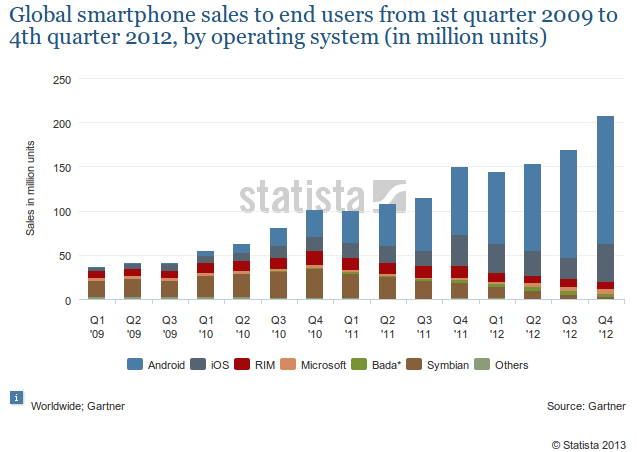
\includegraphics[scale=0.6]{images/sale}
\caption{Verkaufszahlen von Smartphones weltweit nach Plattform}
\label{sale1}
\end{center}
\end{figure}

Aktueller Vorreiter der Brache ist das auf Linux basierende Betriebssystem Android von Google Inc. Die wachsende Beliebtheit dieses Betriebssystems für Tablets und Smartphones macht es umso interessanter für Entwickler. So werden immer mehr Applikationen und Services für Geräte entwickelt, die dieses Betriebssystem nutzen. Die wachsenden Zahl an Software für Android ist in Abbildung \ref*{androidmarket}\footnote{http://de.statista.com/statistik/daten/studie/74368/umfrage/anzahl-der-verfuegbaren-apps-im-google-play-store/} zu erkennen. 

\begin{figure}[h!t]
\begin{center}
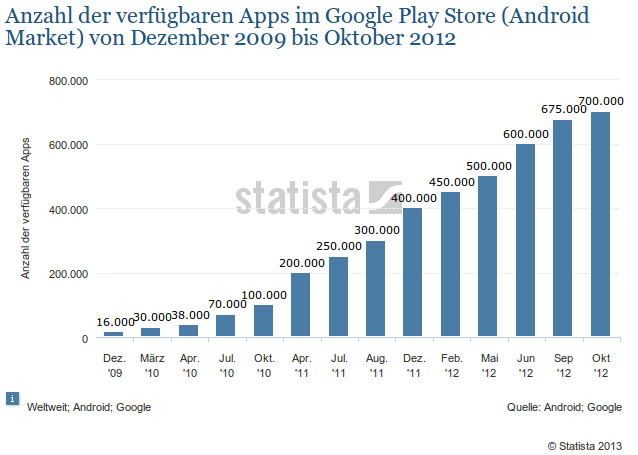
\includegraphics[scale=0.6]{images/androidmarket}
\caption{Anzahl der Applikationen für Android}
\label{androidmarket}
\end{center}
\end{figure}

Um einen Einblick in die Entwicklung von Applikationen für das mobile Betriebssystem zu bekommen, haben wir uns für die Entwicklung einer Applikation für die besagte Plattform entschieden. Diese soll für eine bestimmte Problemstellung konzipiert sein und eine angemessen Lösung darstellen.

\subsection{Vorwort}

Die Arbeit soll Einblicke in die Entwicklung von Applikationen für das Betriebssystem Android gewähren. Es werden die Grundstrukturen vorgestellt und erläutert. Diese sind nötig um die Art und Weise zu verstehen, wie Applikationen auf der Plattform ausgeführt und vom Nutzer verwendet werden können.

Abschließend werden verschiedene Probleme und Lösungswege während den Konzipierung und der Implementierung sowie während der Projektbearbeitung erläutert.

Dies beinhaltet verschiedene projektorganisatorische Elemente wie Versionierung und Projektplanung (\ref{proj}). Die folgenden Abschnitte beschäftigen sich mit der Herangehensweise an die Projektarbeit in kleinen Teams sowie deren Funktionsweise und Anwendung.

Im weiteren Verlauf werden verschiedene Schritte der Konzeptionierung sowie Implementierung verschiedener Komponentenstrukturen der Applikation diskutiert und ausgewertet. Das letztendliche Ziel der Arbeit ist eine nutzbare zweckgerichtete Applikation.

Diese Applikation soll dazu dienen die Grundlagen der Android Plattform zu verstehen. Dies beinhaltet die Funktionsweise von nativen Android Applikationen (\ref{natand}) sowie die des Android SDK. Ein tiefes Verständnis für das eigentliche Android Betriebssystem erleichtert die Entwicklung und das Verständnis über verschiedene betriebssystemspezifische Eigenheiten. Diese und weitere Grundlagen werden ebenso in dieser Arbeit behandelt und diskutiert.
%!TEX root = ../docu.tex
\subsection{Die Architektur von Android}
\subsection{Anwendungsstruktur}
%!TEX root = ../docu.tex
\section{Projektplanung}
\label{proj}

\subsection{Arbeitspakete und Planung}
Bevor man mit der Arbeit an einem Projekt beginnen kann, stellt sich die Frage, wie Programmfeatures implementiert und Fehler beseitigt werden sollen. Außerdem müssen Aufgaben an verschiedene Personen verteilt werden.

Hierfür gibt es viele Vorgehensweisen. Eine der Häufigsten ist das Anfertigen von sogenannten Arbeitspaketen. Diese beinhalten das vorher definierte Ziel und jene Schritte, die zur Erreichung des Ziels nötig sind und welche Anforderungen das Ziel erfüllen muss.

Ein solches Arbeitspaket wird anschließend bewertet und im Aufwand eingeschätzt. Das so erstellte Arbeitspaket wird jetzt einem Bearbeiter zugeteilt.

Abhängigkeiten von Arbeitspaketen oder solche, die aufeinander aufbauen, spielen eine gesonderte Rolle. Schnittstellen zwischen verschiedenen, in den Paketen implementierten Programmkomponenten müssen genau definiert werden, um spätere Fehler oder Inkompatibilität auszuschließen.

Die Verwaltung der Pakete und Zuweisung variiert je nach Größe des Teams. Weit verbreitet sind Systeme wie Trac\footnote{http://trac.edgewall.org/}, Bugzilla\footnote{http://www.bugzilla.org/} oder Redmine\footnote{http://www.redmine.org/}. Für ein Team mit kleinerer Anzahl von Mitgliedern empfehlen sich solche Systeme nicht.

Die Wartung und Konfiguration ist zu aufwendig. Die Kosten von Zeit und entstehender Nutzen stehen in keinem vertretbaren Verhältnis.

Für die Umsetzung des Projektes wurde daher das Managementtool namens Trello\footnote{https://trello.com/} eingesetzt. Es realisiert eine Managementmethode namens \textit{Kanban}, welche von Automobilhersteller Toyota entwickelt wurde.

\subsubsection{Kanban}

Die Funktionsweise von Kanban wird auf ein paar wesentliche Bestandteile differenziert. Zunächst werden Stadien definiert. Je nach Projektumgebung variieren diese Stadien. Für die Entwicklung von Anwendungen sind folgende Stadien ausreichen. 

\begin{itemize}
	\item Zu Beginn ist ein Paket im Stadium \textit{nicht zugewiesen} beziehungsweise \textit{neu}.
	\item Das nächste Stadium ist \textit{zugewiesen} gefolgt von \textit{in Bearbeitung}.
	\item Anschließend wandert das Arbeitspaket in das Stadium \textit{Test} und von dort aus in \textit{beendet}.
\end{itemize}

Das System ist übersichtlich da alle Pakete auf einen Blick einsehbar. Des Weiteren ist ersichtlich, welche Person für das jeweilige Arbeitspaket zuständig ist und es bearbeitet. Durch die Position eines Paketes ist sofort erkennbar, in welchen Stadium sich gerade ein Paket befindet.

Ein positive Eigenschaft von Kanban ist die hohen Transparenz der Arbeitspakete und deren gegenwärtigen Status. Die Einführung und Umsetzung sind ressourcenschonend und schnell. Der Umgang mit Kanban ist leicht zu erlernen und gerade für kleine Teams zu empfehlen.

\begin{figure}
\begin{center}
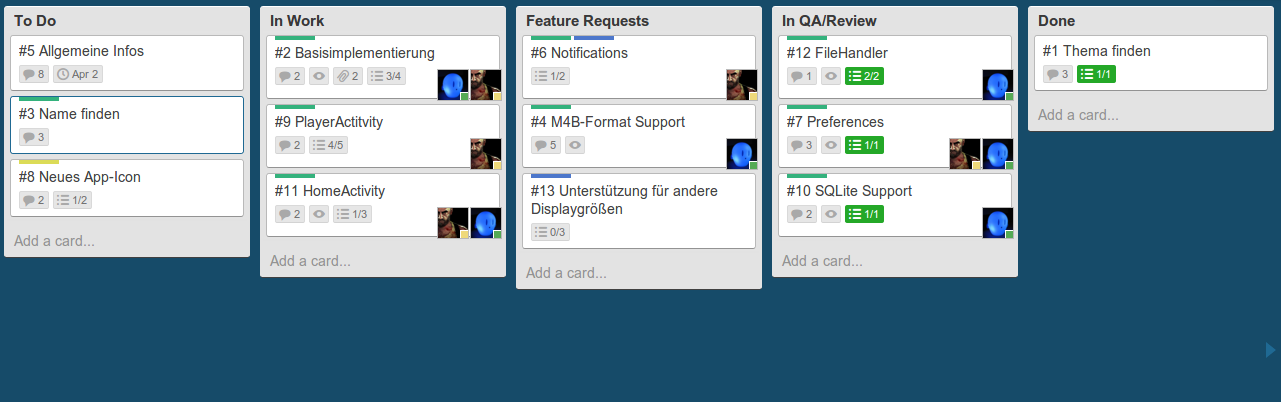
\includegraphics[scale=0.35]{images/kanban}
\caption{Kanbanboard mit verschiedneen arbeitspacketen}
\label{kanban}
\end{center}
\end{figure}

In Abbildung \ref{kanban} ist ein Kanban-Board abgebildet. Aufgaben werden dort auf Karten, die Arbeitspakete repräsentieren, dokumentiert. Diese durchlaufen verschiedene Stadien und wandern von der linken zu rechten Seite des Boards.

Abgeschlossene Pakete werden nach einiger Zeit vom Brett, genommen um die Übersichtlichkeit weiterhin zu gewährleisten. Solche Boards werde in Papierform oder auch auf elektronischen Wege simuliert. Weitere Einzelheiten kann aus der Literaturquelle \cite{9783898647304} entnommen werden.

\subsection{Entwicklungsumgebung}

Für das Arbeiten mit der umfangreichen Android API empfiehlt es sich, eine Entwicklerwerkzeuge wie Eclipse zu verwenden. Dies gewährleistet einen schnellen Umgang mit allen Bestandteilen des Android SDK.

Des Weiteren wird die Auswertung von LOG-Daten durch das SDK schnell und Fehler somit eher identifiziert. Ähnlich wie bei der Entwicklung von Java Anwendungen ist es möglich Test zu implementieren und dadurch Fehlererkennung und dessen Beseitigung zu betreiben.

Eclipse bietet eine automatische Vervollständigung für Quellcode und eine Typprüfung vor der Kompilierung des Codes. Es ist weiterhin in der Lage viele Codeabschnitte automatisch zu erzeugen und somit Entwicklungsschritte zu erleichtern.

Wichtig bei der Arbeit mit einer IDE\footnote{engl. Integrated Development Environment} wie Eclipse ist die Integration des SDKs, um die für die Entwicklung von Android Applikationen bereitgestellten Werkzeuge nutzen zu können. Hierzu gehören verschiedene Debugger sowie Kompilierwerkzeuge, welche dem Entwickler Hilfestellung leisten.

\subsection{Versionsverwaltung des Quellcode}

Die Versionierung von Quellcode spielt eine große Rolle bei der Entwicklung von Software. Hierbei werden Änderungen am Quellcode zeitlich erfasst um einen chronologischen Verlauf von Änderungen festzuhalten und die Aktualität des Codes zu gewährleisten.

Für diesen Zweck gibt es verschiedene Lösungsmöglichkeiten. Weit verbreitet sind die Versionsverwaltungssysteme SVN\footnote{http://subversion.apache.org/} und GIT\footnote{http://git-scm.com/}.
SVN ist ein zentrales Versionsverwaltungssystem für Dateien. Es gibt einen zentralen Versionierungsserver zudem sich Klienten verbinden um Änderungen einzureichen.

Die Wahl für die Versionsverwaltung viel auf GIT. GIT verfolgt eine andere Strategie. Änderungen werden dezentral verwaltet. Im folgenden Kapitel werden die wesentlichen Aspekte von GIT genannt.

\begin{description}

\item[Kein zentraler Server] \hfill \\
Jeder Benutzer hat eine exakte Kopie der Versionierung und ihren Verlauf. Alle Arbeiten werden daher größtenteils ohne Netzwerkzugriff ausgeführt.

\item[Datenaustausch] \hfill \\
Der Austausch von Daten wird über viele Protokolle und Arten abgewickelt. Der Austausch ist sehr flexibel und sicher, wenn für die Übertragung geeignete, abgesicherte Protokolle verwendet werden.

\item[Kryptographische Sicherheit der Projektgeschichte] \hfill \\
Während des Versionierungprozesses wird ein eindeutiger Hash erzeugt, welcher den gesamten Verlauf zur aktuellen Version wiederspiegelt. Eine nachträgliche Änderung ist somit nicht möglich und es ist ausgeschlossen, dass sie verschleiert wird. Gelöschte Informationen bleiben erhalten und können wiederhergestellt werden.
\end{description}

Durch die Dezentralisierung der Versionierung muss dennoch ein Austausch der Daten zwischen den Teammitgliedern gewährleistet werden. Hierfür gibt es verschiedene Möglichkeiten, unter anderem eine gemeinsame Austauschstelle. Diese Austauschstellen fungieren als Vermittel- und Sammelpunkte. Es besteht die Möglichkeit solch einen Punkt selber zu betreiben oder kostenlose Anbieter wie GitHub\footnote{https://github.com/} zu verwenden.
%!TEX root = ../docu.tex
\section{Konzept}

\subsection{Grundkonzept}

Das folgende Kapitel erläutert die Kozeptionierung der Anwendung, welche im späteren Verlauf implementiert wird. Hierbei handelt es sich um eine Applikation die hauptsächlich für das Abspielen von Hörbüchern im Audioformat MP3 genutzt werden soll. Die Applikation ist so ausgelegt, das alle Funktionen einfach erreichbar und bedienbar sind.

Die Applikation soll dem Benutzer ermöglichen Hörbücher abzuspielen, welche er vorher auf sein mobiles Endgerät abgelegt hat. Hierfür muss die Applikation eine Einstellungsmöglichkeit beinhalten. Über diese Einstellung muss der Benutzer den Speicherort wählen und festlegen. Über diesen Einstellungsparameter ist es der Anwendung nun möglich alle Audiodateien aufzulisten und abzuspielen. Die Auflistung filtert alle nicht abspielbaren Daten und ermöglicht des Weiteren in Unterordnen zu navigieren. Ein Element der Liste stellt dabei entweder eine Audiodatei oder ein Unterordner dar. 

\begin{figure}[h!t]
\begin{center}
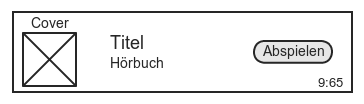
\includegraphics[scale=0.8]{images/listitem}
\caption{Mockup für ein Listenelement}
\label{mocklistel}
\end{center}
\end{figure}

Die Abbildung \ref{mocklistel} beschreibt ein solches Element. Es enthält das Cover des Hörbuches sowie den Titel und die genau Abspielzeit. Aus dieser Auflistung heraus werden alle Audiodateien abgespielt die sich im aktuellen Verzeichnis befinden. Eine Schnittstelle zur Übertragung der Informationen zur Player-Komponente realisiert diese Funktion. Diese Komponente ist für das eigentliche Abspielen zuständig. Sie empfängt die Anweisung zum Abspielen der Audiodatei und spielt dieses Datei ab.

\begin{figure}[ht]
\begin{minipage}[b]{0.45\linewidth}
\centering
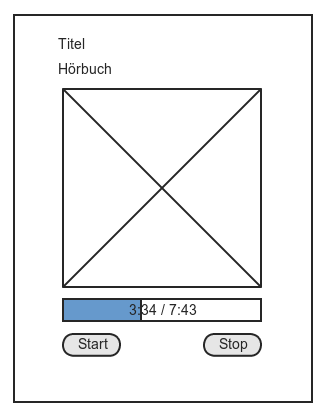
\includegraphics[width=\textwidth]{images/playerkomp}
\caption{Konzept des Players}
\label{playerkomp}
\end{minipage}
\hspace{0.5cm}
\begin{minipage}[b]{0.45\linewidth}
\centering
\fbox{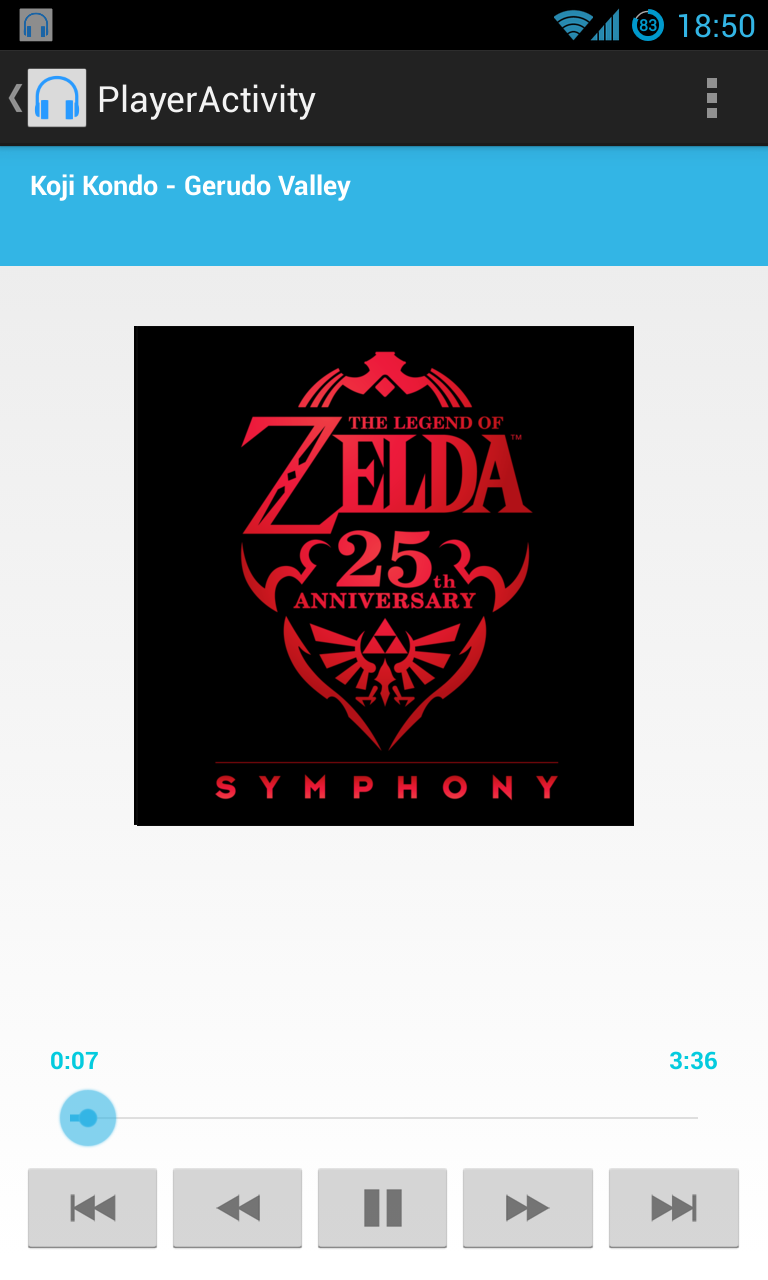
\includegraphics[width=\textwidth]{images/player_unframed}}
\caption{Player-Implementierung}
\label{player}
\end{minipage}
\end{figure}

Die Player-Komponente wie in Abbildung \ref{playerkomp} als Mockup und in Abbildung \ref{player} als realer Screenshot dargestellt, ermöglicht das Abspielen zu steuern. Dies beinhaltet das Stoppen, Pausieren und andere Funktionen. Des Weiteren ist Erkennbarkeit welche Audiodatei abgespielt wird. Eine Vorschrittanzeige lässt erkennen, wie viel von der Audiodatei bisher abgespielt wird sowie die Gesamtlänge der Audiodatei.

\begin{figure}
\begin{center}
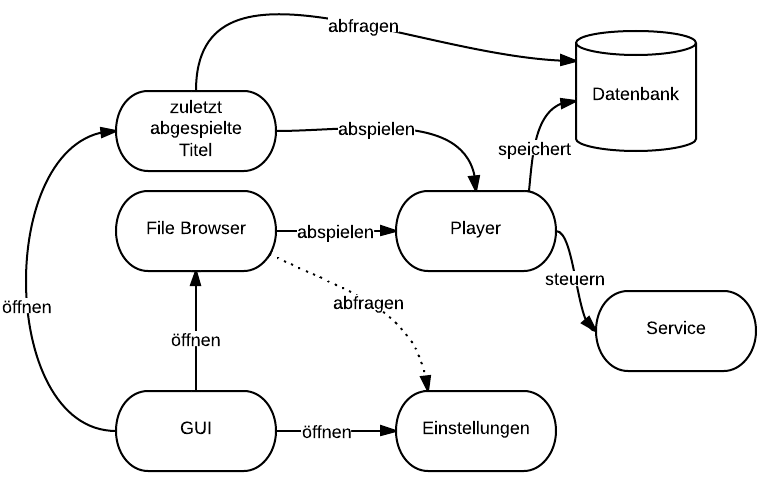
\includegraphics[scale=0.6]{images/konzept}
\caption{Schematische Darstellung der Anwendung}
\label{konzept}
\end{center}
\end{figure}

Wird die Anwendung beendet wird die Wiedergebe abgebrochen. Sie ist in der Lage Abbrüche der Wiedergabe zu erkennen und diese zu speichern. Der Benutzer hat dann die Möglichkeit, die Wiedergabe an diesen Punkten fortzusetzen.

Die Eingabe erfolgt durch ein übliches Touchscreen-Display und ist darauf optimiert. Hierzu gehört klare und einfache Programmstrukturen sowie ausreichend große Flächen für Bedienelemente und Steuerung von Programmfunktionen. Die gesamte Programmstruktur ist so aufgebaut, dass eine Weiterentwicklung und Implementierung neuer Funktionen möglich ist.
%!TEX root = ../docu.tex
\section{Programmstruktur}

\subsection{Allgemeiner Programmaufbau}

\subsubsection{Benutzeroberfläche}

Die Steuerung aller Programmfunktionen wird durch eine Benutzeroberfläche realisiert. Diese Oberfläche wird über die typischen Elemente von Android Smartphones unterstützt. Zum einen sind das die üblichen drei Systemknöpfe und zum anderen die gegen Druck sensible Anzeigefläche\footnote{Touchscreen}.

Die Standard Eingabeknöpfe bei Android Telefonen sind: \textit{Zurück}, \textit{Home} und \textit{Menü}-Knopf. Diese befinden sich auf allen Android basierenden Smartphones. Einige Knöpfe lassen sich zur Steuerung von Programmfunktionen nutzen andere wiederum nicht. Viele neuen Geräte wie zum Beispiel das Nexus 4\footnote{http://www.google.de/nexus/4/} oder Nexus 7\footnote{http://www.google.de/nexus/7/} haben diese Knöpfe softwaretechnisch integriert. Das heißt sie werden durch Teile des Displays realisiert.

Der Hauptteil der Steuerung erfolgt über die gegen Druck sensible Anzeigefläche des Telefons. Der Aufbau solcher Displays variiert je nach Hersteller und Typ. Die Funktion unterscheidet sich nicht. Das Display erfasst die Druckpunkte von Fingern auf dem Display. Diese Impulse werden in Koordinaten umgerechnet um Interaktionen mit dem Elementen auf dem Display zu ermöglichen. Die errechneten Koordinaten entsprächen jenen die sich unmittelbar unterhalb des Druckpunktes befinden.

Durch diese Interaktion können verschiedene Bedienelemente verwendete werden. Diese reichen von Buttons über Listen die durchlaufen werden können und so weiter.

\subsubsection{Mediaplayer}

Das Abspielen von Audiodateien wird von einen Mediaplayer realisiert. Dieser erhält als Eingabeparameter eine Audiodatei. Der Pfand dieser Audiodatei dient zur Identifizierung und wird für das Abspielen benötigt.

Der Player ist so konzipiert das eine Liste alle Audiodateien im Ordner, indem sich die übergebene Audiodatei befindet erzeugt wird. Diese Liste ist gleichzeitig die Warteschlange des Mediaplayers.

Der Mediaplayer muss nicht eigenständig implementiert werden. Die Android API bietet einen schon implementierten Player für verschiedene gängige Audioformate wie MP3\footnote{ISO/IEC 11172-3, ISO/IEC 13818-3} an. Alle benötigten Decoder-Werkzeuge sind im Player integriert. Für spezielle Audioformate müsste eine passende Erweiterung implementiert oder ein anderer Player verwendet werden.

\subsubsection{Datenbankstrukturen}
\label{Datenbankstrukturen}

Viele moderne Anwendungen benötigen Speicherbereiche um anfallende Anwendungsdaten aus dem Hauptspeicher aus zu lagern. Diese Daten sollen jedoch für einen späteren Zugriff leicht erreichbar bleiben und von anderen Anwendungen nicht manipuliert werden können.

Für diesen Zweck gibt es mehrere Möglichkeiten. So ist es zum Beispiel denkbar anfallende Anwendungsdaten zu Verschlüsseln und zusammen mit den Nutzerdaten auf den internen oder externen Telefonspeicher ab zu legen. Diese Daten sind nun durch Dritte manipulierbar. Dies beeinträchtigt die Stabilität und Sicherheit der eigenen Anwendung und des gesamten Systems.

Um nun Entwickler die Speicherung von Anwendungsdaten zu erleichtern, ist es möglich durch die Android API eine integrierte Datenbank zu verwenden. Diese bietet nicht nur Schutz der eigenen Daten vor anderen Anwendungen, sondern auch vor dem Anwender selbst.

Als Datenbank Struktur wird das quelloffene Datenbank-Management-System SQlite\footnote{http://www.sqlite.org/} verwendet. Es ist sehr ressourcensparend und einfach in die Programmstruktur einzubinden. Während der Laufzeit der Anwendung verbraucht der Datenbankserver (DBMS\footnote{Datenbankmanagementsystem}) nur wenige hundert Kilobyte vom Hauptspeicher.

Alle anfallenden Daten werden in einer einzigen Datei gespeichert. SQlite bietet alle wichtigen Features wie Tabelle, Views, Trigger usw. Es gibt jedoch auch Unterschiede, so ist es zum Beispiel nicht möglich mehre Schreib- und Leseprozesse parallel auszuführen. Alle Datenbankoperation werden daher sequenziell ausgeführt. SQlite biete keine Typsicherheit, fehlerhafte Eingaben werden einfach umgewandelt und gespeichert. Dies ist bei der Entwicklung von Anwendungen zu beachten.

Somit hat jede Anwendung welche die SQlite Datenbank implementiert hat, eine eigene separate und vor anderen Anwendungen Geschütze Datenbank.

Daten werden mittels SQL-Syntax abgefragt. Anders als bei vielen Datenbankserver verfügt SQlite keine Benutzer und Zugriffskontrolle. Es gelten die Schrieb- und Leserechte des Dateisystems. Es ist weiterhin nicht möglich Tabellen im vollen Umfang zu verändern, so wie man es von herkömmlichen relationalen Datenbanken gewohnt ist. Der SQL-Befehlt \textit{ALTER TABLE} ermöglicht das Umbenennen von Tabellen und hinzufügen von Spalten.

SQlite ist durch seine einfache Struktur und Handhabung das meistgenutzte Datenbanksystem der Welt.
%!TEX root = ../docu.tex
\section{Entwicklung}

\subsection{Benutzeroberfläche}

Die Interaktion von Benutzer und Programmstrukturen erfolgt über eine Benutzeroberfläche oder auch GUI\footnote{engl. Graphical User Interface}. Diese ist besonders einfach gehalten um eine intuitive Bedienung des Programms zu gewährleisten.

\begin{figure}[h!t]
\begin{center}
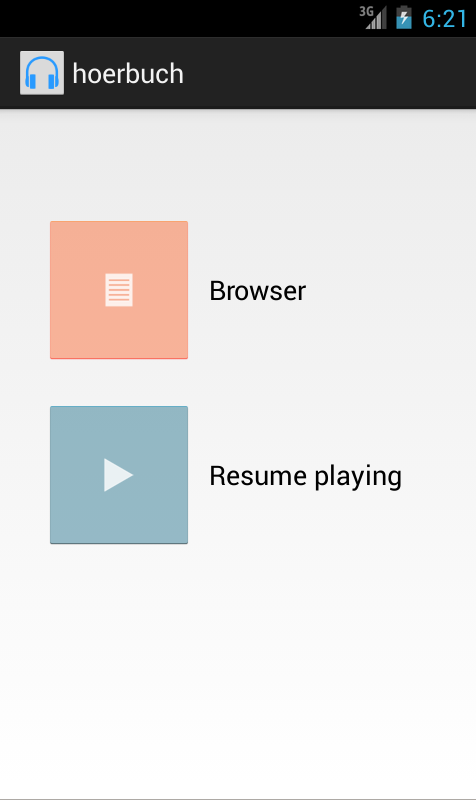
\includegraphics[scale=.2]{images/mainscreen}
\caption{Hauptansicht der Anwendung}
\label{mainscreen}
\end{center}
\end{figure}

Position und Größe von Elementen und Bedienstrukturen sind so gewählt, dass die Eingabe über das Display so einfach wie möglich ist. Über eine Hauptansicht gelangt der Benutzer zu allen benötigten Funktionen der Anwendung. Diese Ansicht ist in Abbildung \ref{mainscreen} dargestellt.

Die Farbgebung orientiert sich am Holo-Design von Android. Dieses Design wird durch klare Farbgebung in Schwarz und Blau charakterisiert. Die Hauptfunktionen beinhalten zum einen die Auswahl einer bestimmten Audiodatei und zum anderen das Wiederaufnehmen von abgebrochenen Wiedergaben. Beide Funktionen werden über durchlaufbare Listen dargestellt und variieren nur minimal vom Design. Dennoch sind es zwei unterschiedliche Funktionen.

\begin{figure}[h!t]
\begin{center}
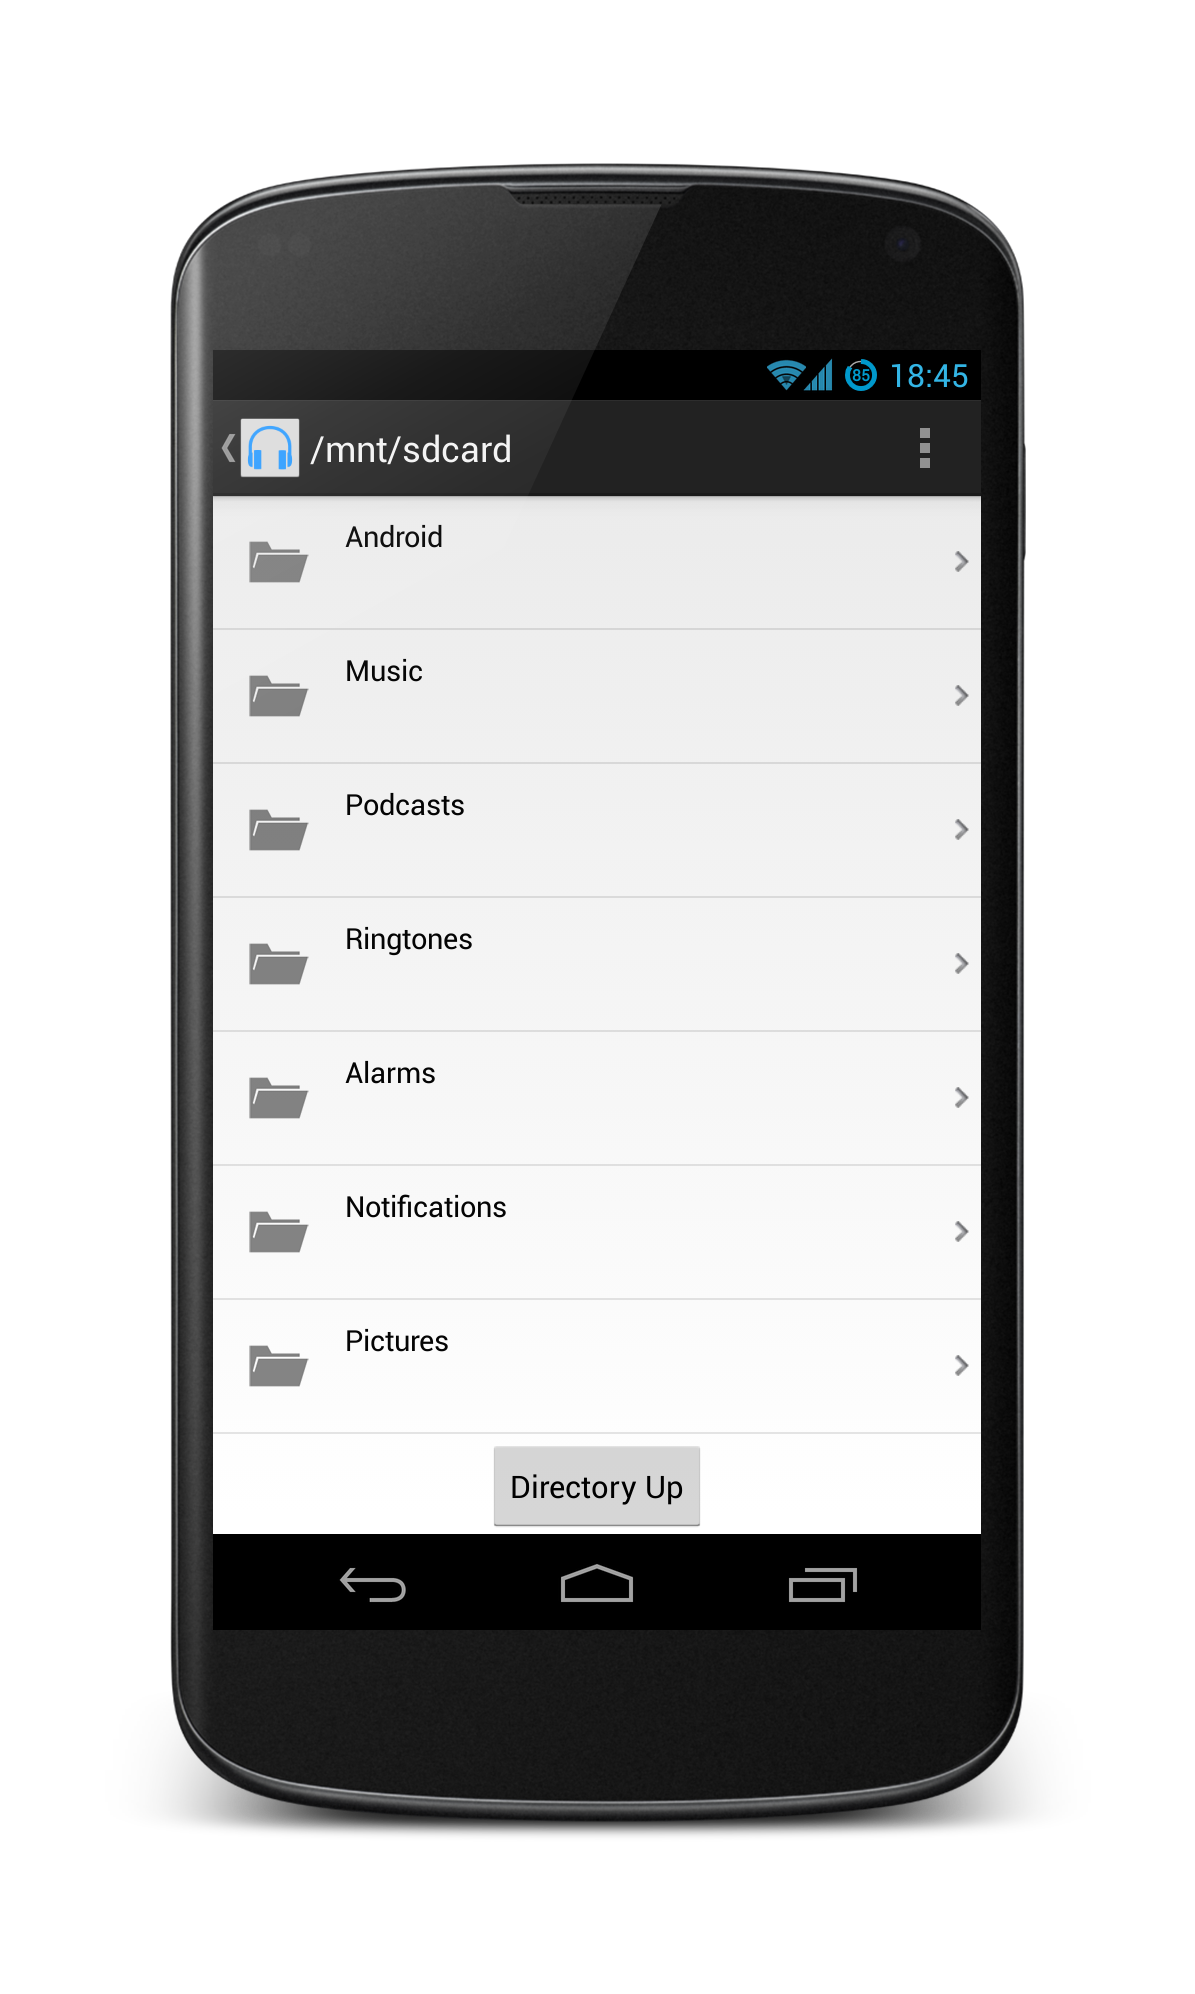
\includegraphics[scale=.2]{images/browsing}
\caption{Auswahl der Audiodatei durch Liste}
\label{browsing}
\end{center}
\end{figure}

Abbildung \ref{browsing} zeigt die Auswahlmöglichkeit über die Listenansicht. In Abbildung \ref{broken} ist die Liste mit den abgebrochenen Wiedergaben zu erkennen.

\begin{figure}[h!t]
\begin{center}
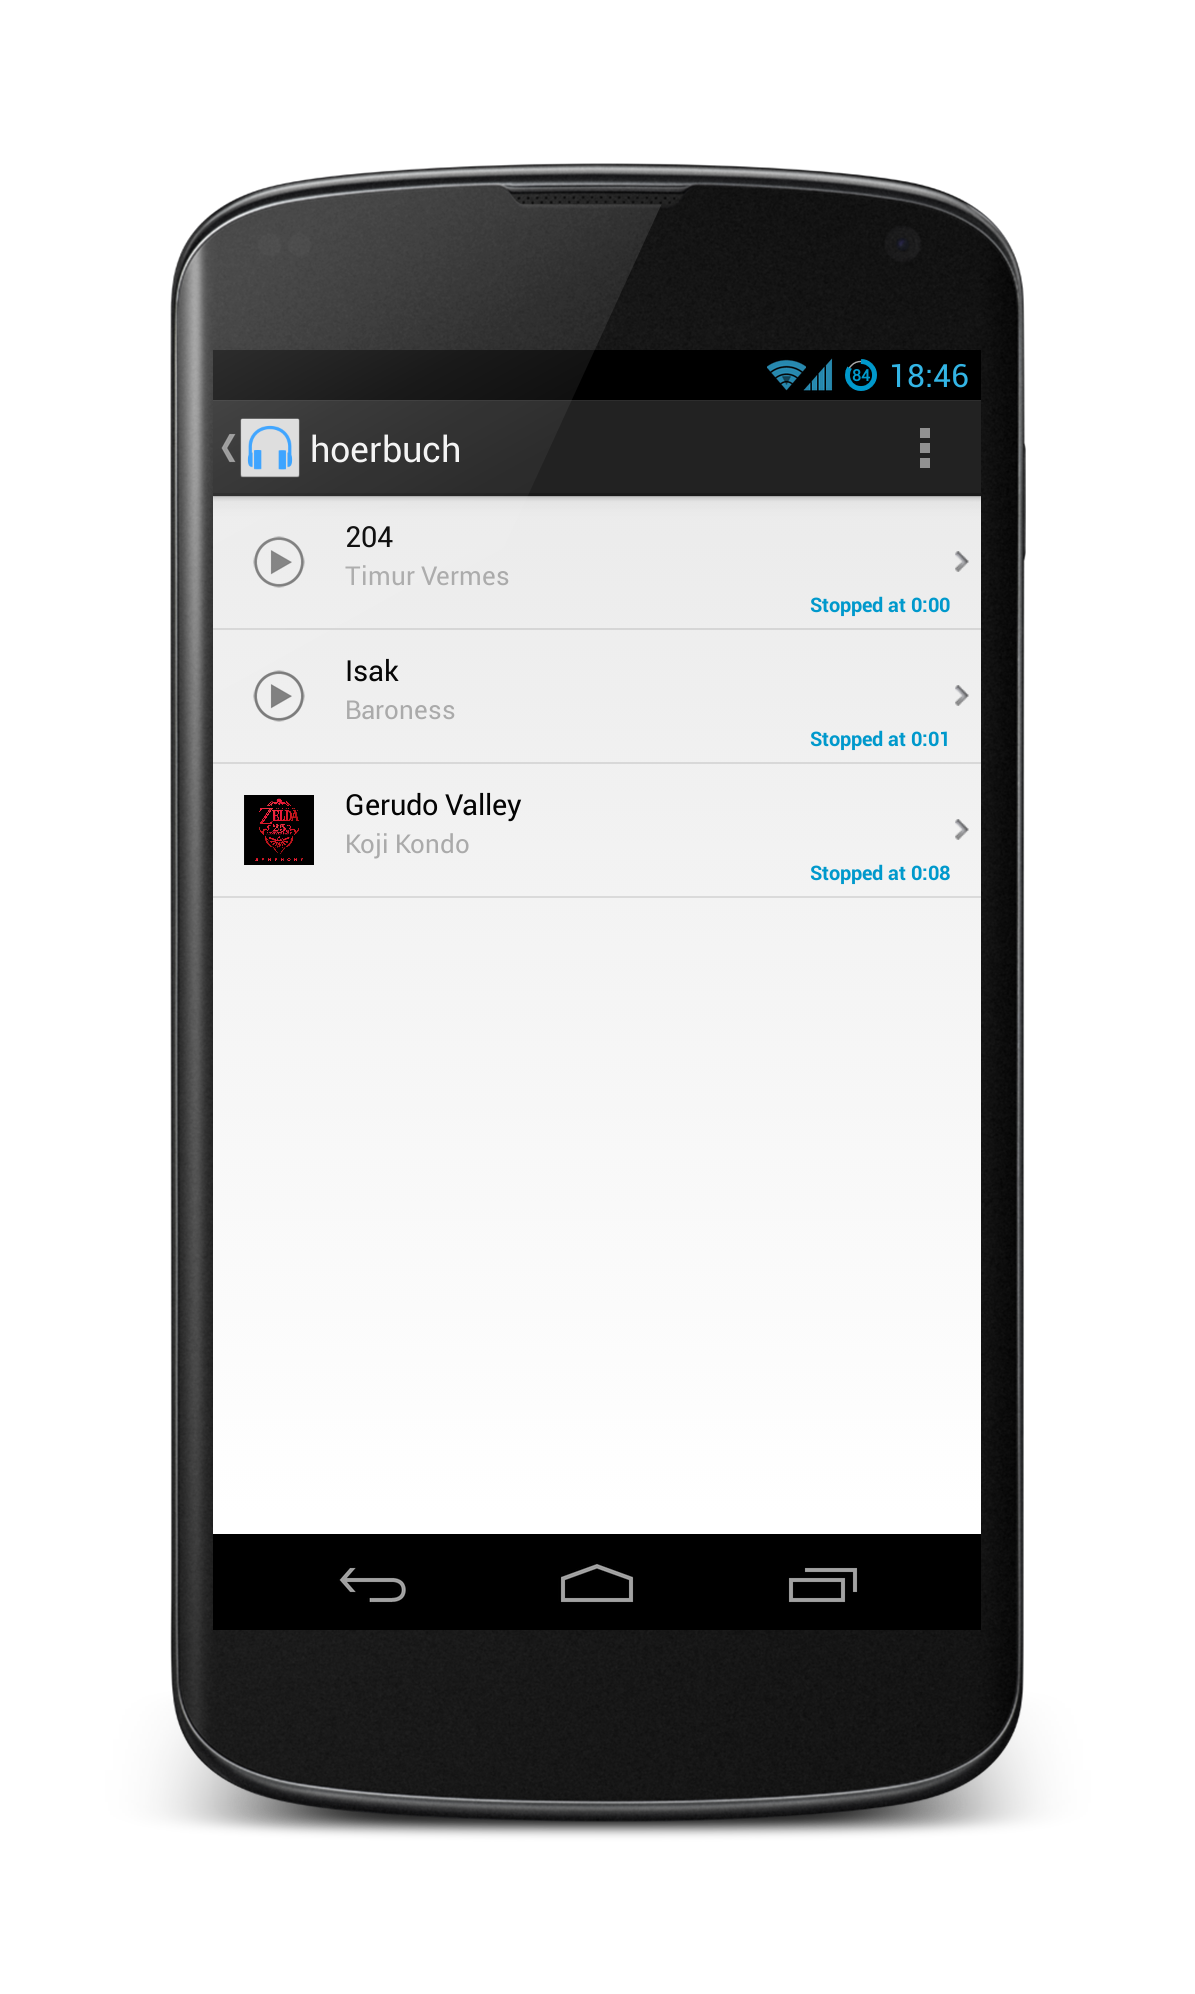
\includegraphics[scale=.2]{images/broken}
\caption{Liste mit abgebrochenen Wiedergaben}
\label{broken}
\end{center}
\end{figure}

Das Auswählen der Audiodateien oder Wiederaufnehme erfolgt über einfache Eingaben über das Display mit Druck auf das jeweilige Element in der Liste.

Die Einstellung der Anwendung wird über die \textit{Menü}-Taste aufgerufen. Alle Funktionen bilden eigene Strukturen und sind durch separate Klassen definiert. Diese Struktur soll in den nachfolgenden Unterkapiteln von \ref{classes} behandelt werden.

\subsection{Klassenstruktur}
\label{classes}

Um ein Gesamtbild über die Struktur des Projektes zu geben werden im folgenden Abschnitt die Klassen vorgestellt und zusammengefasst, die eine wichtige Funktion in der Anwendung übernehmen.

\subsubsection{Activities}

Als erstes werden in Abbildung \ref{cd_activities} die Activities vorgestellt. Wie in Abschnitt \ref{components} beschrieben, stellen Activities die sichtbaren Bildschirminhalte dar. Methoden die Android standardmäßig benötigt und durch das Interface \verb+Activity+ bereitgestellt werden sind einmal \verb+onCreate()+ die aufgerufen wird, wenn die Activity gestartet wurde. Weiterhin sind \verb+onCreateOptionsMenu()+, was für die Darstellung des Optionsmenüs notwendig ist, und \verb+onOptionsItemSelected()+, welches Aktionen für die Optionen definiert, in jeder Activity enthalten.

\begin{figure}[ht!]
\begin{center}
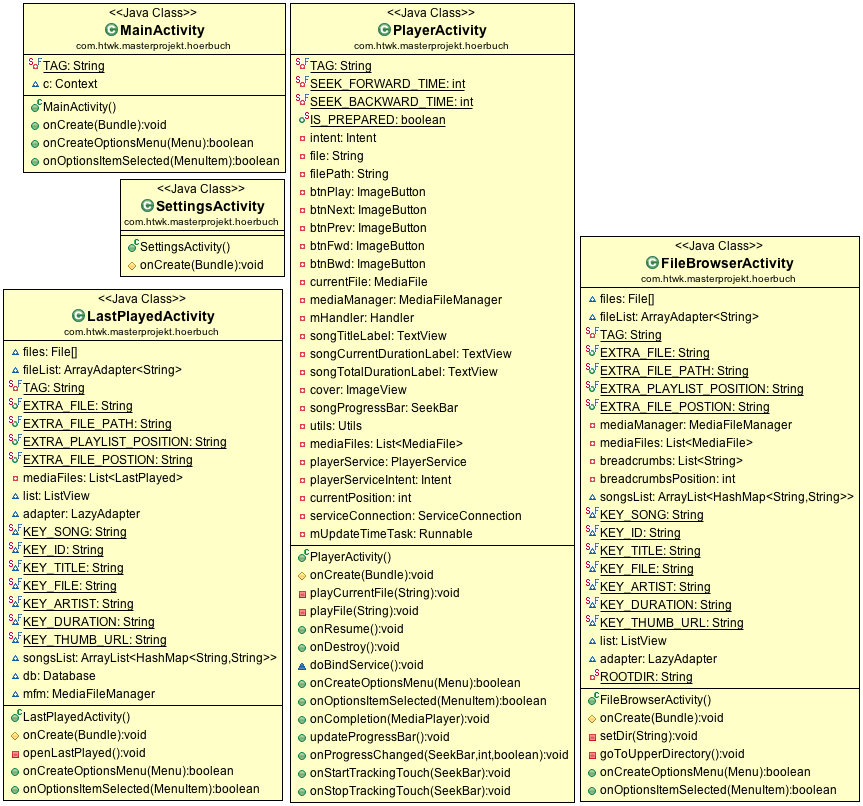
\includegraphics[scale=.5]{images/diagram}
\caption{Klassenübersicht der Activities}
\label{cd_activities}
\end{center}
\end{figure}

Die Activities selbst haben dabei folgende Aufgaben:

\begin{description}[style=nextline]
	\item[MainActivity] Wird angezeigt, wenn die Applikation gestartet wird. Außer den beiden Buttons für das Starten der \verb+FileBrowserActivity+ und der \verb+LastPlayedActivity+ befindet sich darauf nichts.
	\item[SettingsActivity] Stellt das Einstellungsmenü dar. Da die Inhalte dieses Menüs an anderer Stelle per XML definiert werden befinden sich keine weiteren Methoden in der Klasse.
	\item[FileBrowserActivity] Wird angezeigt, wenn man auf den \emph{Browser}-Button im Hauptmenü klickt. Hier wird der Dateibrowser angezeigt über den die Hauptnavigation durch die Hörbücher und Ordner möglich ist.
	\item[LastPlayedActivity] Stellt den Browser dar, der die letzten gehörten Hörbücher anzeigt. Man kommt in diese Ansicht, wenn man im Hauptmenü den entsprechenden Button drückt.
	\item[PlayerActivity] Der eigentliche Hörbuch-Player. Dieser wird gestartet, wenn man eine Datei im Browser ausgewählt hat.
\end{description}

\subsubsection{Die MediaPlayer-Architektur}

\begin{figure}[ht!]
\begin{center}
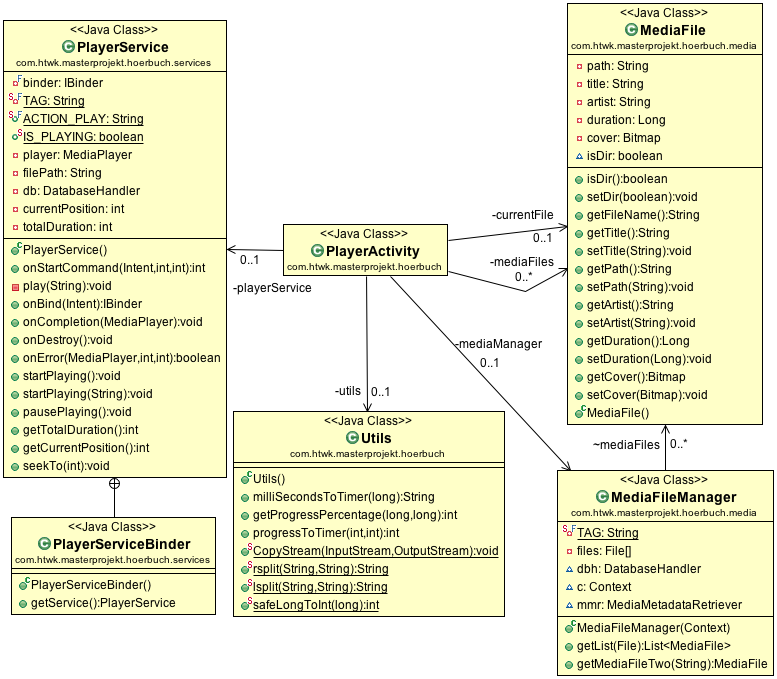
\includegraphics[scale=.5]{images/cd_media}
\caption{Klassenübersicht der MediaPlayer-Architektur}
\label{cd_media}
\end{center}
\end{figure}

Um Mediadateien abspielen zu können stellt die Android-Plattform die Klasse \verb+MediaPlayer+ zur Verfügung. Um ein Hörbuch abzuspielen wird die gewählte Datei geladen und vorbereitet. Das übernimmt der \verb+PlayerService+. Die Entscheidung dies in einen Service, einen gesonderten Thread auszulagern ist damit begründbar, dass das vorbereiten der Datei bei großen Datein den Haupt-Thread in dem das User-Interface läuft blockiert und die Anwendung träge macht. Gerade im Bereich der Hörbücher muss der Player mit Dateien bis zu \SI{1}{GB} zurechtkommen. Durch die Auslagerung in den Service kann das Hörbuch im Hintergrund vorbereitet werden, ohne, dass der Nutzer eine Verzögerung der Oberfläche mitbekommt.

Wie in Abbildung \ref{cd_media} zu sehen, bildet die \verb+PlayerActivity+ das Zentrum.Ausgehend davon befindet sich der \verb+PlayerService+ und der \verb+PlayerServiceBinder+ welcher die Kommunikation zwischen dem Service und der Activity unterstützt.

Um eine Mediendatei ausreichend gut zu repräsentieren wurde die Datenstruktur \verb+MediaFile+ implementiert. Diese enthält alle Daten die für den Player zum Abspielen oder zur Darstellung von Informationen notwendig sind. 

Der \verb+MediaFileManager+ hat die Aufgabe Dateien vom Speicher zu lesen. Dabei extrahiert er dessen Metainformationen und speichert diese zusammen mit dem Pfad als Liste von \verb+MediaFile+. Diese Liste kann vom Browser oder vom Player als Playlist verwendet werden. Damit nur Dateien gelesen werden, die auch wirklich abgespielt werden können, wird der \verb+AudioFilter+ verwendet. Dieser filtert vorher definierte Dateitypen und vermeidet unnötiges Lesen von nicht abspielbaren Dateien.

Die Klasse \verb+Utils+ bietet verschiedene Werkzeuge an die unter anderem für die Darstellung notwendig sind. So können damit beispielsweise die vom MediaPlayer ausgegebenen Millisekunden in ein lesbares Format umgewandelt werden.

\subsection{Einstellungen}

Das Einstellungsmenü soll in jedem Zustand der Applikation erreichbar sein. Der einzige Ort an dem dies möglich ist, ist das Menü. Hier ist nicht von einem implementierten Menü die reden. Dieses Menü ist in jeder Applikation erreichbar und wird durch das Betriebssystem bereitgestellt.

Drückt ein Benutzer die Menü-Taste, welche sich an jedem Gerät befindet, welches Android als Betriebssystem verwendet, so öffnet sich eine Menü-Schnittstelle. Diese wird durch den Entwickler mit Einträgen befüllt und kann dadurch bestimmte Funktionen bereitzustellen. Eine typische Funktion ist die Einstellungsseite.

Die Konfiguration der Einstellungsmöglichkeiten, welche dem Nutzer zur Verfügung gestellt wird, erfolgt über eine XML Datei. In älteren API-Versionen wurde dies noch durch Klassen realisiert. Diese Klassen und Methode sind in den Version ab Android Version 4 veraltet und sollten nicht mehr verwendet werden.

Die erwähnte XMl-Datei wird nun durch bestimmte Regler und Kontrollstrukturen bestückt. Diese Strukturen werden durch IDs\footnote{Identifier} validiert. Ihre Werte können durch eine Abfrage aus der Anwendung heraus ausgelesen werden.

Sollten keine geeigneten vorgefertigte Kontrollstrukturen wie zum Beispiel Radio-Button oder Checkboxen vorhanden sein, so können eigene Strukturen eingebettet werden.

Im konterten Projekt existiert keine Struktur für das Speichern und Durchsuchen eines Ordnerpfades. Dieser \textit{FilePicker} wurde daher eigens implementiert und kann aus dem Einstellungsmenü aufgerufen werden.

\begin{center}
\begin{figure}
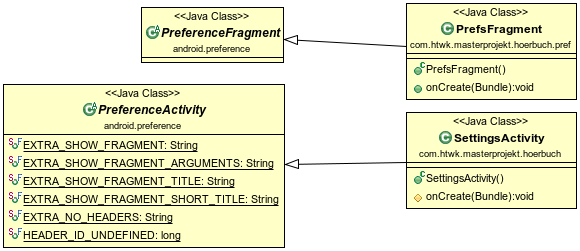
\includegraphics[scale=0.7]{images/settings}
\caption{Klassen für die Implementierung der Einstellungen}
\label{settings}
\end{figure}
\end{center}

Wurde der gewünschte Ordner gefunden, kann dieser in den Einstellungen gespeichert werden. Alle anderen Komponenten der Anwendung können nun auf diese Einstellungen zugreifen.

Dies wird über den \textit{PreferenceManager} realisiert. Er benötigt für die Abfrage des Wertes lediglich die ID der Einstellung. Die angesprochene ID hat einen Wert hinterlegt welche bei der Abfrage zurückgegeben wird. Zur Sicherheit wird bei der Abfrage ein Standartwert angegeben, im Falle das die Einstellung nicht gefundene oder ausgelesen werden konnte. Die einmal eingetragen Einstellungen sind jederzeit abrufbar und auch nach Beenden der Applikation immer noch vorhanden.

Die Abbildung \ref{settings} zeigt die benötigten Klassen für die Implementierung der Funktionalität der Einstellungen.

\subsection{Datenbank}

\subsubsection{Grundlagen}

Das Android eine Schnittstelle für SQlite Datenbanken anbietet, wurde schön in einem vorherigen Kapitel \ref{Datenbankstrukturen} behandelt. Anschließend wird nun erläutert wie man diese Anbindung benutzt und wie Daten gespeichert und abgefragt werden.

Zunächst benötigen wir eine Klasse welche die API-Klasse \textit{SQLiteOpenHelper} erweitert. Diese bildet nun die Schnittstelle unser Applikation und der Datenbank, welche wir benutzen möchten bzw. anlegen möchten.

Jeder Applikation ist es möglich mehrere Datenbanken anzulegen und zu verwenden. Um Datenbanken voneinander unterscheiden zu können, werden die einzelnen Datenbanken über Namen verifiziert und aufgerufen.

Um Android mitzuteilen, welche Datenbank wir öffnen möchten, wird dem Betriebssystem mitgeteilt 
um welche Applikation es sich handelt und wie der Name der zu öffnenden Datenbank ist.

Das Resultat ist eine Verbindung zu einer SQlite Datenbank. Um Daten zu speichern, wird eine Tabellen angesprochen. Diese Tabelle wir bei der Erstellung der Datenbank mit anlegen.

Für diesen Zweck legen wir eine Methode mit den Namen \textit{onCreate} an. Diese Methode wird beim Erstellen der Datenbank ausgeführt und enthält alle SQL-Befehle zum Anlegen der von uns gewünschten Tabellen.

Sollte sich das Datenbankschema ändern kann dies über eine weiter Variable, welche wir dem Betriebssystem mitteilen realisiert werden. Eine Datenbankversion beschreibt den Stand der Datenbankstruktur. Sollte sich die Datenbankstruktur geändert haben wird die Versionsnummer erhöht und eine andere Methode wird beim anbinden zur Datenbank aufgerufen.

\begin{figure}
\begin{center}
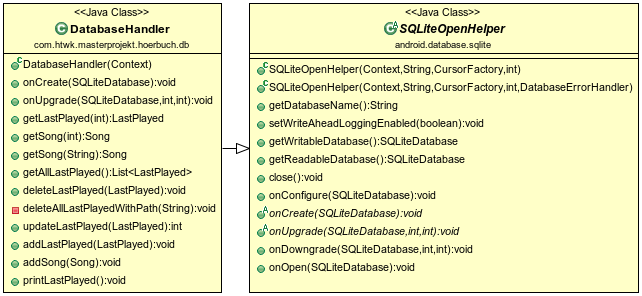
\includegraphics[scale=0.7]{images/database}
\caption{Klassen für die Implementierung der Datenbank}
\label{database}
\end{center}
\end{figure}

Diese Methode nennt sich \textit{onUpgrade} und wird bei eben erwähnter Erhöhung der Versionsnummer automatisch ausgeführt. In dieser Methode sollten eine Datenmigration durchgeführt werden oder alle bestehenden Daten gelöscht werden und neue Tabellen angelegt werden.

Durch diesen Mechanismus ist die Aktualität des Datenbanklayouts immer gegeben. In der Abbildung \ref{database} sind die Klassen ersichtlich, die es ermöglichen mit der Datenbank zu kommunizieren. Für die Verwendung der Daten ist es ratsam Objekte zu verwenden um abgefragte Datensätze weiter zu verwenden. Ein solches Objekt wird in Abbildung \ref{dbmodel} dargestellt.

\begin{figure}
\begin{center}
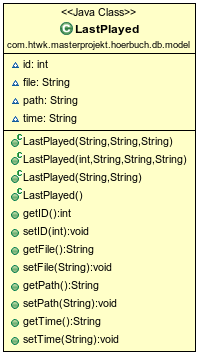
\includegraphics[scale=0.7]{images/dbmodel}
\caption{Obejkt zum transport der datensätze}
\label{dbmodel}
\end{center}
\end{figure}

\subsubsection{Abfragen}

Eine Datenbankabfrage wird über einen SQL-Befehl an die Datenbank gestellt. Mit dem Befehl \textit{SELECT} und der Angabe der Tabelle können Daten aus der Datenbank abgefragt werden. Die Abfrage wird dafür in eins Cursor-Objekt geladen und der Cursor anschließend zur Ausführung an die Datenbank gesendet.

Das Cursor-Objekt enthält anschließend alle abgefragten Daten, welche die Datenbank zum übergeben SQL-Befehl gefunden hat. Eine direkte Abfrage ist nicht möglich.

Es muss immer eine Cursor-Objekt verwendet werden. Möchte man nur bestimmte Daten oder zielgerichtet Datensätze aus der Datenbank laden, wird dem Cursor-Objekt eine Filterung mitgeteilt, welche von der Datenbank bei der Abfrage der Daten berücksichtigt wird.

Das Cursor-Objekt enthält eine Liste von allen Dateneinträgen die gefunden wurde. Sind mehre Datensätze gefunden wurden, können diese durchlaufen werden und jeder Datensatz einzeilig betrachtet und verarbeitet werden.

Bei der Abfrage der einzelnen Felder des Datensatzes ist es nötig den Datentyp der einzelnen Daten zu kennen. Das Cursor-Objekt hat verschiedene Methoden um unterschiedliche Datentypen aus den Feldern zu lesen. Diese Typen können wie schon erwähnt nicht typsicher abgefragt werden. So ist es möglich ein Datenfeld des Types \textit{Integer} in eine variable des Typen \textit{String} zu laden.

Der Zugriff der Datenbank kann nur schreibend oder lesend gewährt werden. Eine Kombination ist nicht möglich. Ein Zugang zur Datenbank kann entweder nur schreibend oder lesend sein.

Möchte man Schrieben und Lesen, wird dies durch einen schreibenden Zugriff und anschließen über einen lesenden Zugriff realisiert. Diese beiden Vorgänge müssen separat initiiert werden.

\subsubsection{Löschen}

Das Löschen von Daten erfolgt ebenso wie das Selektieren durch SQL-Befehle. Anders wie bei dem Selektieren existiert hierfür kein Cursor-Objekt. Es wird lediglich mitgeteilt welcher Datensatz in welcher Tabelle gelöscht werden soll.

\subsubsection{Ändern}

Ähnlich verhält es sich mit den Ändern von Datensätzen. Hierfür wird der Datenbank mitgeteilt, welcher Datensatz geändert werden soll und welche Datenfelder mit welchem Wert gesetzt werden soll.

Die Referenzierung einzelner Datensätze erfolgt über Primärschaltregler oder andere Datenfelder, welche im SQL-Befehl angegeben werden müssen.

\subsubsection{Einfügen}

Das Anlegen neuer Datensätze wird durch die Methode \textit{insert} ausgelöst. Diese Methode verlangt ein Liste von Schlüssel-Wert-Paaren um einen Datensatz anlegen zu können.

Die Liste von Paaren repräsentiert den eigentlichen Datensatz. In ihr werden alle Datenfelder und die dazugehörigen Werte abgelegt. Ausgeschlossen ist der Primärschlüssel, dieser wird durch einen Trigger in der Datenbank automatisch erzeugt und beim Einfügen in die Datenbank an den Datensatz abgehangen und gespeichert. Der Methode wird nun die Liste mit den Daten übergeben und die Tabelle genannt, in der die Daten abgelegt werden soll. Der Trigger muss nicht separat angelegt werden, sondern wird durch das Erzeugen einer Spalte, welche als Primärschlüssel gekennzeichnet wird, angelegt.
%!TEX root = ../docu.tex
\section{Fazit}

\subsection{Aufgetretene Probleme}

Während der Entwicklung sind einige Probleme aufgetreten. An diese Stelle wird auf diese genauer eingegangen und die Lösung für das aufgetretene Problem diskutiert.

\subsubsection{Laufzeiten für verschiedene Operationen}

Die Laufzeit spielt in Anwendungen für Benutzer eine große Rolle. Langsame Laufzeiten wirken frustrieren auf Benutzer und die Akzeptanz für lange Wartezeiten ist gering. Diese langen Laufzeiten treten häufig bei rechenintensiven Operationen auf. Eine dieser Operation ist das Erzeugen von Vorschaubildern, welche aus MP3 Dateien extrahiert werden, um sie in der Auswahl für die jeweiligen Titel anzuzeigen.

Die Extraktionen benötigen zunehmen Zeit je mehr Titel hintereinander analysiert werden müssen. Die Lösung hierfür ist satt jede MP3 im Ordner zu analysieren, wird ein Verweis in einem Bildcache für den jeweiligen Ordner hinterlegt. Die Gründe hierfür sind zum einen das dadurch nur eine Extraktion durchgeführt werden muss und zum anderen ist dies möglich da zusammengehörige MP3 meist im gleichen Ordner abgelegt sind und nicht mit anderen Fremden gemischt werden.

Ein ähnliches Problem tritt bei der Extraktion von Metadaten wie zum Beispiel der Interpret des Albums oder Titel der Audiodatei auf. Für diese Operation muss für jede Audiodatei eine lese Aktion ausgeführt werden. Eine Lösung hierfür konnte nicht implementiert werden und eine höhere Laufzeit wurde daher in Kauf genommen. Eine mögliche Lösung ist es einen komplette Erfassung aller Audiodateien vorzunehmen und alle Informationen der Metadaten in einer Datenbank abzulegen.

\subsubsection{Hintergrundprozesse}

Eine weiter Problemstellung war es, die Wiedergabe in einem Hintergrundprozess zu versetzen, sodass wehrend der Wiedergabe andere Aktionen und Anwendungen auf dem Gerät gestartet und verwendet werden können. Hierfür bietet die API von Android gewisse Services an, welche in ein Hintergrundprozess versetzt werden können und so die angesprochene Problemstellung gelöst wird.

Wichtig bei der Arbeit mit Threads und Services ist der Austausch von Daten und Zugriff auf gemeinsame Speicherbereiche.

\subsection{Ergebnisse}

Das Ergebnis der Gemeinschaftsarbeit ist eine funktionsfähige Applikation die den gesteckten Anforderungen des Konzeptes genügt. Die Anwendung bietet Raum für Erweiterungen und Verbesserungen. Dabei wurde darauf geachtet das Programmerweiterungen problemlos in den Programmcode eingeführt werden kann ohne schon bestehende Programmfunktionen zu blockieren oder zu zerstören.

Die Projektstruktur wurde einfach gehalten um Quellcodefragmente wiederverwenden zu können oder Weiterentwicklung betreiben zu können. Die Entwicklung von nativen Anwendungen ist aufwendig. Der Vorteil bestimmte Systemkomponenten nutzen zu können überwiegt dennoch.

Durch die Arbeit am Projekt wurden die Grundlage für die Entwicklung für native Anwandelungen für Android Plattformen angeeignet und erprobt. Des Weiteren sind Kenntnisse über die Android Plattform und des Android Betriebssystem erarbeitet und angelernt wurden. Das Arbeiten in kleineren Gruppen erfordert flexible und einfache Kommunikationsstrukturen. Diese unterschiedene sich stark von Projekten in größeren Gruppe wie etwa die Scrum\cite{9783868998337} Projektarbeit.

\newpage
\bibliography{literatur}
\bibliographystyle{abbrv}
\end{document}
